
\subsection{Robustness}
I run a number of difference tests to confirm the validity of my findings. First I run a placebo regression using two periods of data before the introduction of mobile money to check the validity of the common trends assumption. Then I run an IV regression to further control for any potential self-selection into mobile money use. Lastly I use propensity score matching to match mobile money users with a sample of non users who are as similar as possible on observed baseline characteristics. I use this matched sample to re-run my earlier results and  confirm their validity. All three of these tests confirm my earlier results and support their implications.   

\subsubsection{Placebo test}
The placebo test allows me to check that future mobile money use does not predict past changes in consumption, thus confirming the common trends assumption required for a difference-in-difference specification to be valid. I run a placebo test using the 2007 Tanzanian Household Budget survey (HBS) combined with the NPS 2008-9 wave 1  to construct two rounds of data prior to the introduction of mobile money services. A subsample of the 2007 HBS was re-sampled in the NPS, so by combining this sample with the first wave of the NPS I created a panel of 1,200 households covering 2 periods before the introduction of mobile money, which I call wave 0 (2007) and wave 1 (2008-9). I created a dummy variable for whether the household ever uses mobile money after it's introduction in 2009 and I use this to estimate the following equation: 
\begin{align} \label{eq: placebo}
C_{jit} = &  \gamma_a AggShock_{jvt} + \mu MME_{jvt}      + \beta_m MME_{jvt}\cdot AggShock_{jvt}  \notag \\
& + \bm{\theta X_{jvt}} +  \bm{\psi X_{jvt}} \cdot AggShock_{jvt} +  \alpha_j + \varepsilon_{jvt} 
\end{align}
where $MME_{jvt}$ is a dummy variable equal to zero in wave 0 and one in wave 1 if the household uses mobile money in the future. If the common trends assumption holds then the dummy for future mobile money use will not be significant for the past data, confirming that it is not unobservable characteristics of places that get mobile money agents or households which choose to use mobile money that is driving my results. 

The HBS includes different compositions of goods in the measure of non-food consumption (for example in the inclusion and depreciation of durable assets) and hence is not directly comparable to the expenditure measure used in the NPS. I therefore look only at food consumption per capita when I estimate \eqref{eq: placebo} . I constructed the same measures of control variables to match those used for in the main analysis such as household head education, household size and occupation dummies and summary statistics for these are shown in the appendix Table \ref{placebo_sum}. Unfortunately some variables were not recorded in the HBS, such as detailed financial data, since the survey was principally aimed at measuring poverty and so did not ask as rich a set of questions as the NPS. The HBS didn't ask questions on the number of loans a household had, bank account use or membership of a ROSCA. In comparing the placebo test to my main result I therefore re-run \eqref{eq: specification agg shock} using only per capita food consumption and with the same set of controls available in the HBS to make the results as comparable as possible. These are recorded alongside the placebo test. The rainfall shock variable used here is a self-reported drought or flood. This information was asked in the NPS for the last 5 years so I was able to create a shock dummy for the 2007 data. \begin{table}
\centering
\caption{Placebo test of future mobile money use 2007-2009} \label{placebo}

\begin{tabular}{lccccc} \multicolumn{5}{c}{Dependent variable: Log food consumption per capita} \\\hline
& \multicolumn{2}{c}{Placebo pre-mobile money data} & \multicolumn{2}{c}{Actual mobile money use data} \\ \cmidrule(r){2-3} \cmidrule(l){4-5}
 & (1) & (2) & (3) & (4) \\
 & Diff-in-diff & FE & Diff-in-diff  & FE \\ \hline
 &  &  &  &  &  \\
Rain shock &-0.05** & -0.04 & -0.07***  & -0.04 \\
 & (0.03) & (0.05) & (0.03)  & (0.04) \\
 MM ever & -0.04 & -0.05 &    &  \\
 & (0.05) & (0.05) &  &  &  \\
MM use &  &  & 0.06** & 0.06** \\
 &  &  & (0.03) & (0.03) \\
 
Rain shock*MM ever & 0.01 & 0.01 &  &  \\
 & (0.09) & (0.01) &  &  \\

Rain shock*MM use &  &  & 0.11**  & 0.12** \\
 &  &  & (0.05) & (0.06) \\
Observations & 2,332 & 2,332 & 9,567  & 9,567 \\
Number of individuals & 1,204 & 1,204 & 3,738 & 3,738 \\
R-squared & 0.369 & 0.225 & 0.276  & 0.101 \\
  \hline
\multicolumn{5}{p{14cm}}{Regressions include clustered errors at the village level and a reduced set of control variables consisting of: household head age, household head education, female head dummy, household size, rural dummy, whether the household owns a mobile phone, baseline wealth level constructed from principal component analysis and household head occupation dummies. The shock variable here is a self-reported drought or flood dummy. Regressions (1) and (2) run specification \eqref{eq: placebo} on 2007 and 2008-9 data with a dummy variable MM ever if a household ever used mobile money after 2009 and regressions (3) and (4) run specification \eqref{eq: specification agg shock} on the three waves of NPS data. MM use is a dummy variable equal to one if the household uses mobile money in a given year.} \\
\multicolumn{5}{l}{ Standard errors in brackets, *** p$<$0.01, ** p$<$0.05, * p$<$0.1} \\
\end{tabular}
\end{table}

The results in Table \ref{placebo} show the placebo test in columns (1) and (2) alongside the equivalent regressions of actual mobile money use on food consumption per capita and with the same set of control variables in columns (3) and (4). I find that food consumption reacts to rainfall shocks in the simple difference-in-difference specifications, though less strongly than total expenditure did, perhaps because households are likely to protect the smoothing of food over other forms of consumption after a shock. There is no differential effect for households which use mobile money in the future in their consumption or ability to respond to a shock in the past. This lends support to the common trend assumption necessary for using a difference-in-difference specification and suggests the emergence of a significant relationship between the ability to smooth shocks and mobile money is due to the use of mobile money and not another variable.   

\subsubsection{IV regressions}
If mobile money use is endogenous to household's ability to smooth consumption due to self-selection of households into mobile money use then my results will be biased. I can use instrumental variable regression to control for this. Given there are two potentially endogenous variables, mobile money use and the shock interaction with mobile money use, I need two instruments. An instrument would need to be correlated with mobile money use (relevant) but not affect consumption smoothing independently (exogenous). 

An instrument that has also been used in the literature is distance to the nearest mobile money agent. Distance to the nearest agent is correlated with mobile money use since it is easier to use mobile money if an agent is nearby. And it shouldn't be correlated with unobserved determinants of the ability of households in a village to smooth risk. In addition to the distance to the nearest agent I also have a variable of the cost of transport to the mobile money agent. This is the monetary cost by public transport to the nearest mobile money agent. The straight line distance to the nearest agent may not be an accurate measure of the difficulty of getting to that agent which will depend on the availability of good roads and a source of transport there. The correlation between distance to the agent and cost to get to the agent is 0.71, so while the two variables are correlated with each other they are not perfectly so. I therefore instrument with the distance and cost to the nearest mobile money agent and the interactions of distance and cost to the nearest mobile money agent with the rainfall shock. 

\begin{table}
\centering
\caption{IV results} \label{IV}
\begin{tabulary}{0.9\textwidth}{Lcccc} 
\multicolumn{5}{c}{Dependent variable: Log consumption per capita}\\\hline
& \multicolumn{2}{c}{Self reported shock} & \multicolumn{2}{c}{1 sd rain shock} \\
 & (1) & (2) & (3) & (4) \\
 \cmidrule(r){2-3} \cmidrule(l){4-5}
 & IV Diff-in-diff & IV FE & IV Diff-in-diff & IV FE \\ \hline
 &  &  &  &  \\
Rain shock & -0.10*** & -0.09** & -0.05 & -0.06*  \\
 & (0.04) & (0.04) & (0.05) & (0.04)  \\ 
Village MM use & 0.47 & 0.22 & 0.40 & 0.28* \\
 & (0.43) & (0.21) & (0.72) & (0.16) \\
Mobile money use & -0.44 & -0.05 & -0.46 & -0.10 \\
 & (0.84) & (0.37) & (1.67) & (0.42) \\
 Rain shock*MM use & 0.14 & 0.13 & 0.31 & 0.09  \\
 & (0.14) & (0.13) & (0.33) & (0.16)  \\
Observations & 5,367 & 4,862 & 5,367 & 4,862 \\
Number of individuals & 2,431  & 2,431 & 2,431 & 2,431 \\
R-squared & 0.49 & 0.12 & 0.50 & 0.12 \\\hline
F-stat on excluded instruments for MM use & 6.87 & 11.83 & 8.35 & 10.62 \\
F-stat on excluded instruments for Rain shock*MM use & 38.12 & 37.09 & 106.5 & 118.7 \\
Cragg-Donald Wald F statistic & 6.23 & 7.68 & 6.47 & 6.40 \\
Underidentification test $\chi^2$ p-value & 0.00 & 0.00 & 0.00 & 0.00 \\
Sargan-Hansen test $\chi^2$ p-value & 0.49 & 0.74 & 0.21 & 0.50\\\hline
\multicolumn{5}{p{13cm}}{ Instruments were distance and cost to nearest mobile money agent and their interactions with the shock variable. All regressions include full set of household control variables from Table \ref{HH sum}. Village MM use refers to the proportion of households in the village using mobile money. Mobile money use is a dummy variable equal to one if that household uses mobile money. }\\
\multicolumn{5}{l}{ Standard errors in brackets, *** p$<$0.01, ** p$<$0.05, * p$<$0.1} \\
\end{tabulary}
\end{table}

The instrumental variable results in Table \ref{IV} confirm that the rainfall shock has a significant negative effect on consumption per capita of between 5 and 10\%, and is significant at at least the 10\% level in 3 of the regressions. Mobile money mitigates the effect of a shock by on average 10\%, and in one case 30\%, but none of these are significant. Mobile money use has a negative impact on per capita consumption  but is also not significant in any of the regressions. Village mobile money use has a positive effect and is significant at the 10\% level for one regression, with 1/3 of the village using mobile money increasing per capita consumption by 10\%. 


The underidentification test is a LM test of whether the instruments are correlated with the endogenous variables. The null hypothesis is that the equation is underidentified and this is distributed as a chi-squared distribution. The null is rejected for all my regressions. 

The Sargan-Hansen test is an over-identification test which determines if the instruments are exogenous (uncorrelated with the error term). Since I have 4 instruments (cost and distance to the nearest agent and their interactions with the shocks) and 2 endogenous variables I can perform an over-identification test to test the validity of the set of instruments. The null hypothesis is that the instruments are uncorrelated with the error term and and then the test statistic is distributed as chi-squared. Since my errors are clustered, the Hansen J statistic is reported and allows errors to be clustered within villages. I cannot reject the null hypothesis that all my instruments are valid for any of the regressions. 

The F-statistics on the first stage regressions for mobile money use are low suggesting my instruments are weak. A weak instrument means that the explanatory power of the instrument is not enough to allow the coefficient of interest in the second stage regression to be determined. Having weak instruments results in a potentially large bias in my results. The Cragg-Donald Wald F statistic is used to test the strength of more than one excluded instruments. For the IV regressions to have less than 5\% of the bias of OLS then the critical value for the F-statistic is 13.43. All my Cragg-Donald Wald F-statistics are less than this critical value meaning my IV results should be interpreted with caution due to their potential bias. Weak instruments also result in large standard errors as seen in my results. Secondly I am trying to instrument for two endogenous variables which also results in a loss of precision and hence high standard errors. 

Overall though, my IV results cannot reject my main findings and provide support for my results alongside the placebo test and propensity score matching. 

\subsubsection{Propensity score matching}
I use propensity score matching to run equation \eqref{eq: specification agg shock} on a sample of mobile money users and non-users (in villages without mobile money) matched on their observable covariates. Propensity score matching was originally proposed by \cite{rosenbaum1983} to reduce the bias in estimated treatment effects with observational data sets. Matching involves constructing an artificial comparison group using observable characteristics so that for every treated (user of mobile money) observation there is an untreated (non-user of mobile money) one as similar as possible in observable characteristics. It requires the strong assumption that there are no unobservable differences between the treatment and artificial control group also correlated with their ability to smooth risk.    
Propensity score matching constructs a probability that a household will use mobile money based on observable characteristics. This is done by running a probit regression on mobile money use on the set of observable baseline characteristics. The probability that a household uses mobile money conditional on its characteristics can be expressed as: 
\begin{equation}
\Pr(\mathbf{x})=\Pr[P=1|\mathbf{X=x}]
\end{equation}
where $P=1$ for households using mobile money and 0 otherwise, and $\mathbf{X}$ is a vector of characteristics. The propensity scores are then used to match the mobile money users with the corresponding non-users with the closest score, thereby constructing an artificial control group as similar as possible to the mobile money users. 


For the matching, I use nearest neighbour matching with replacement, where each mobile money user is matched to its nearest neighbour non-user based on the propensity score. These closest non-users are the comparison group and are used to produce an estimate of the counterfactual. Propensity score matching therefore tries to mimic the random assignment to treatment and control group by choosing a sample for the control group with the most similar propensities to the treatment group. Replacement increases the accuracy of the matching but reduced the number of non-users used to match the users, therefore increasing the variance of the coefficients. Each matched non-user is assigned a frequency weight equal to the number of users it is matched to.

I then use these frequency weights as the weights in a difference-in-difference regression as in \eqref{eq: specification agg shock}. These are reported in Table \ref{pscore}. The results are similar to my main findings in Table \ref{MM spill}. Village mobile money use has a significant effect on household per capita consumption, with $1/3$ of the village using mobile money increasing per capita consumption by 4\%, smaller than the effect seen in my main results. As in the main results there is no benefit from other people in the village  using mobile money when a shock occurs. Own mobile money use is significant in all the regressions which contrasts to my earlier results when there was no effect of own mobile money use in the fixed effects regressions once village mobile money use was accounted for. The interaction of the rainfall shock with mobile money use is significant in three of the regressions and results in per capita consumption improving between 6 and 19\%. However, only two of the rainfall shocks are negative and significant. This suggests that in a matched sample, there is more benefit to own money money use than seen in the unmatched sample, though overall these results support my main findings. 

\begin{table}
\centering
\caption{Regressions using weights from nearest neighbour propensity score matching} \label{pscore}

\begin{tabulary}{0.9\textwidth}{LCCCC} \hline 
\multicolumn{5}{c}{Dependent variable: Log per capita consumption}\\\hline
  & \multicolumn{2}{c}{Self reported rainfall shock} &\multicolumn{2}{c}{ 1sd rain shock} \\ 
 & (1) & (2) & (3) & (4)  \\
  & Diff-in-diff  & FE & Diff-in-diff  & FE \\ \hline

Rain shock & -0.08* & -0.02 & -0.03  & -0.05** \\
 & (0.04) & (0.05) & (0.03) & (0.02)   \\
Village MM & 0.04 & 0.11** & 0.00 & 0.13** \\
 & (0.06) & (0.05) & (0.04)  & (0.05) \\
Rain shock*village MM & -0.05 & -0.04 & 0.04 & 0.03  \\
 & (0.12) & (0.12) & (0.04)  & (0.04) \\
MM use & 0.08*** & 0.06** & 0.08***  & 0.09*** \\
 & (0.03) & (0.02) & (0.02) & (0.02) \\
Rain shock*MM use & 0.12** & 0.06 & 0.19***  & 0.12*  \\
 & (0.05) & (0.05) & (0.07)  & (0.07)  \\
Observations & 3,848 & 3,848 & 3,838  & 3,838 \\
Number of individuals & 1,551 & 1,551 & 1,574 &  1,574 \\
R-squared & 0.57 & 0.13 & 0.57  & 0.12 \\\hline
\multicolumn{5}{p{12cm}}{ Difference-in-difference and difference-in-difference with household fixed effects regressions using frequency weights from nearest neighbour propensity score matching. Village clustered standard errors in brackets and full set of control variables from Table \ref{HH sum}. Village MM refers to the proportion of households in the village using mobile money. MM use is a dummy variable equal to one if that household uses mobile money. The top 5\% of the consumption distribution had been truncated since there are no households in the non-user sample with incomes that high.} \\
\multicolumn{5}{l}{ *** p$<$0.01, ** p$<$0.05, * p$<$0.1} \\
\end{tabulary}
\end{table}  

 Propensity score matching relies on common support of the characteristics of mobile money users and non-users. This requires there to be sufficient overlap of the baseline characteristics of users and non-users of mobile money to make a reasonable comparison between them. I check the common support assumption using a histogram as shown in figure \ref{common_support}. There are fewer observations for non-users at high propensity scores, though common support for the entire distribution.  

\begin{figure}[h]
\centering
\caption{Histograms of common support}
\begin{subfigure}[h]{0.4\textwidth}
\caption{Histogram of common support }
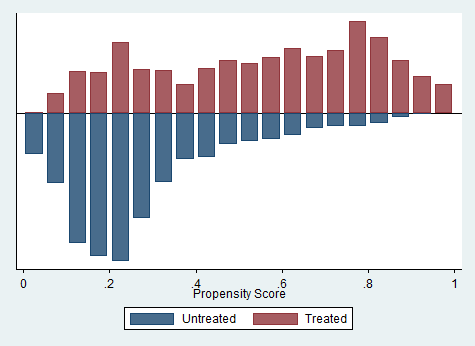
\includegraphics[width=\textwidth,trim= 0.5cm 0cm 0.5cm 0.5cm, clip=true, keepaspectratio]{common_support} \label{common_support}
\end{subfigure}

\end{figure}

To check the common support in more details I conduct balance tests, shown in Table \ref{balance}, on the matched characteristics of users and non-users of mobile money. This table reports the mean values for each covariate for users and non-users of mobile money both before and after matching was done. The t-test tests the null hypothesis that the mean value of the variable is equal for the two groups. Even after matching there are differences between users and non-users across some characteristics. In particular, per capita consumption is not equal after the match, with mobile money users always having slightly higher consumption even after matching. I look at two tests of the overall match balance, Rubins' B and R, where Rubins' B is the absolute standardised difference of the means of the linear index of the propensity score in the treated and (matched) non-treated group) and Rubin's R is the ratio of treated to (matched) non-treated variances of the propensity score index. \cite{rubin2001} suggests that the B value should be less than 25 and the R value between 0.5 and 2. However, after matching my B value is  still 42 which is higher that ideal. My Rubins' R value is within the range suggested for a good match at 1.02. To correct for the higher per capita consumption of mobile-money-using households even after matching, I truncate the top 5\% of the consumption distribution and run my results only for the remaining 95\% of the consumption distribution. 



\begin{table}[!ht]
\centering
\resizebox{!}{0.5\textheight}{\begin{minipage}{\textwidth}
\centering
  \caption{Balance test for propensity score matching} \label{balance}
    \def\arraystretch{0.7}
    \begin{tabulary}{1\textwidth}{lCCCCC}
    \toprule
   
     &       & MM users & Non-users & t statistic  & p statistic  \\
    \midrule
    Per capita  & U     & 13.51 & 13.02 & 74.90 & 0.00   \\
        consumption  & M     & 13.51 & 13.36 & 20.70 & 0.00   \\
    
    Wealth & U     & 1.21  & -0.91 & 68.50 & 0.00    \\
          & M     & 1.15  & 1.48  & -10.90 & 0.051    \\
    Rural & U     & 0.49  & 0.79  & -65.80 & 0.00    \\
          & M     & 0.48  & 0.46  & 5.90 & 0.23   \\
    Education of  & U     & 5.96  & 3.90  & 60.10 & 0.00   \\
        head (yrs)  & M     & 5.95  & 5.97  & -0.40 & 0.94   \\
    Head female & U     & 0.22  & 0.27  & -10.70 & 0.01   \\
          & M     & 0.22  & 0.19  & 21.30  & 0.94    \\
    Age of head & U     & 43.76 & 47.36 & -24.40 & 0.00  \\
          & M     & 43.76 & 46.12 & -13.20 & 0.001    \\
    Household  & U     & 5.13  & 5.18  & -2.00 & 0.64   \\
    size      & M     & 5.13  & 5.37  & -8.20  & 0.059    \\
    Own mobile & U     & 0.70  & 0.28  & 92.30 & 0.00   \\
          & M     & 0.70  & 0.70  & 0.20  & 0.96   \\
    Number of  & U     & 0.11  & 0.05 & 16.80 & 0.00   \\
      loans    & M     & 0.11  & 0.06  & 12.10 & 0.01   \\
    Bank  & U     & 0.00  & 0.00  & .     & .      \\
        account  & M     & 0.00  & 0.00  & .     & .      \\
    ROSCA & U     & 0.07  & 0.02  & 24.40 & 0.00  \\
          & M     & 0.07  & 0.07  & -1.00 & 0.86   \\
     Agriculture/  & U     & 0.44  & 0.74  & -64.20 & 0.00   \\
        Livestock  & M     & 0.44  & 0.40  & 8.30  & 0.09   \\
     Fishing & U     & 0.01  & 0.02  & -8.60 & 0.05  \\
          & M     & 0.01  & 0.01  & 1.70  & 0.64   \\
     Mining & U     & 0.00  & 0.00  & 5.70  & 0.13   \\
          & M     & 0.00  & 0.00  & 2.00  & 0.71 \\
     Tourism & U     & 0.00  & 0.00  & .     & .     \\
          & M     & 0.00  & 0.00  & .     & .     \\
     Employed:  & U     & 0.10  & 0.03  & 25.40 & 0.00   \\
        Gov  & M     & 0.10  & 0.09  & 0.90  & 0.87   \\
     Parastatal & U     & 0.01  & 0.00  & 9.10  & 0.02   \\
          & M     & 0.01  & 0.01  & 4.90  & 0.34   \\
     Private  & U     & 0.14  & 0.04  & 35.40 & 0.00   \\
      sector    & M     & 0.14  & 0.14  & -0.70 & 0.89   \\
     NGO/ & U     & 0.01  & 0.00  & 10.80 & 0.01   \\
       religious   & M     & 0.01  & 0.03  & -13.80 & 0.05   \\
     Employed   & U     & 0.02  & 0.03  & -3.80 & 0.37 \\
       w employees   & M     & 0.02  & 0.02  & 1.40  & 0.74   \\
     Employed   & U     & 0.22  & 0.09  & 37.90 & 0.00   \\
         no employees & M     & 0.22  & 0.26  & -11.50 & 0.41   \\
    Family  & U     & 0.01  & 0.01  & -0.30 & 0.94   \\
       work   & M     & 0.01  & 0.01  & -2.30 & 0.64   \\\hline
         
    \multicolumn{6}{p{10cm}}{Matching was done on wave 1 characteristics. U is for the unmatched sample and M stands for the matched sample}
    \end{tabulary}%
    \end{minipage}}
\end{table}%


\clearpage
